\overlays{3}{%
\begin{slide}{Das Fahrerinterface}
  \begin{minipage}{7.5cm}
    Gr�nde f�r einen PDA:
    \begin{itemstep}
    \item Gen�gend Rechenleistung (Verwendung von Hochsprachen)
    \item Display (Tacho, Warnhinweise etc.)
    \item Interaktion (Einstellungen, Routing, etc.)
    \end{itemstep}
  \end{minipage}
  \begin{minipage}{3cm}
    \center
    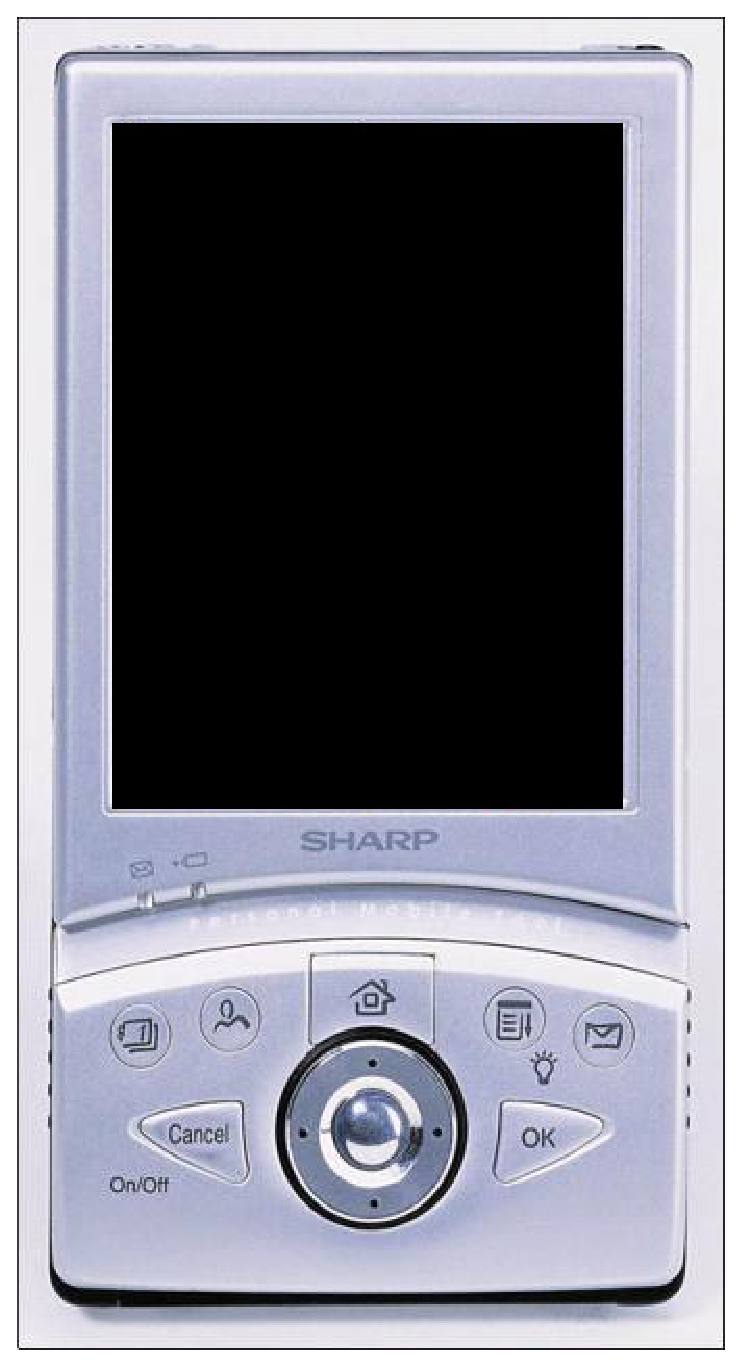
\includegraphics[width=3cm]{zaurus.eps}
  \end{minipage}
\end{slide}
}

% ====================

\begin{slide}{DPI f�r die Entwickler}
  Vaterklasse \texttt{Driver} f�r alle Treiber
  \begin{itemstep}
  \item Methode \texttt{send(Message)} zum Verschicken von \emph{Nachrichten}.
  \item Methode \texttt{receive(Message)} zum Empfang von Nachrichten.
  \end{itemstep}
\end{slide}

\overlays{3}{%
\begin{slide}{Weg der Nachricht durch das DPI}
  \begin{itemstep}
  \item \texttt{Driver.send()} �berpr�ft die Nachricht
  \item \texttt{message\_dispatcher.send()} sendet auf passendem
    \texttt{bus\_manager} heraus $\to$ Indirektion
  \item \texttt{bus\_manager.send()} sendet auf passendem
    \texttt{bus} heraus $\to$ Indirektion
  \end{itemstep}
\end{slide}
}

